%%%%%%%%%%%%%%%%%%%%%%%%%%%%%%%%%%%%%
% Introducción %
%%%%%%%%%%%%%%%%

\section{Introducción}

Existe un consenso generalizado dentro de la comunidad robótica de que los enjambres robóticos serán una herramienta fundamental en el futuro. Una vez esta tecnología alcance su madurez, permitirá llevar a cabo misiones críticas y persistentes, sobre todo en grandes espacios de terreno, o que requieran de una especial resiliencia y abaratamiento de costes, especialmente en términos logísticos y de mantenimiento.

Para entender correctamente a lo que nos referimos cuando hablamos de enjambres de robots, basta con fijarnos en la propia naturaleza. En ella existen numerosos organismos que colectivamente multiplican sus capacidades, generando comportamientos emergentes para resolver tareas que de forma individual pueden resultar muy complejas (ver \autoref{fig:enjambre_naturaleza}). Dichos comportamientos suelen ser muy beneficiosos para el grupo, siempre y cuando la interacción local entre vecinos sea adecuada.

\begin{figure}[h]
    \centering
    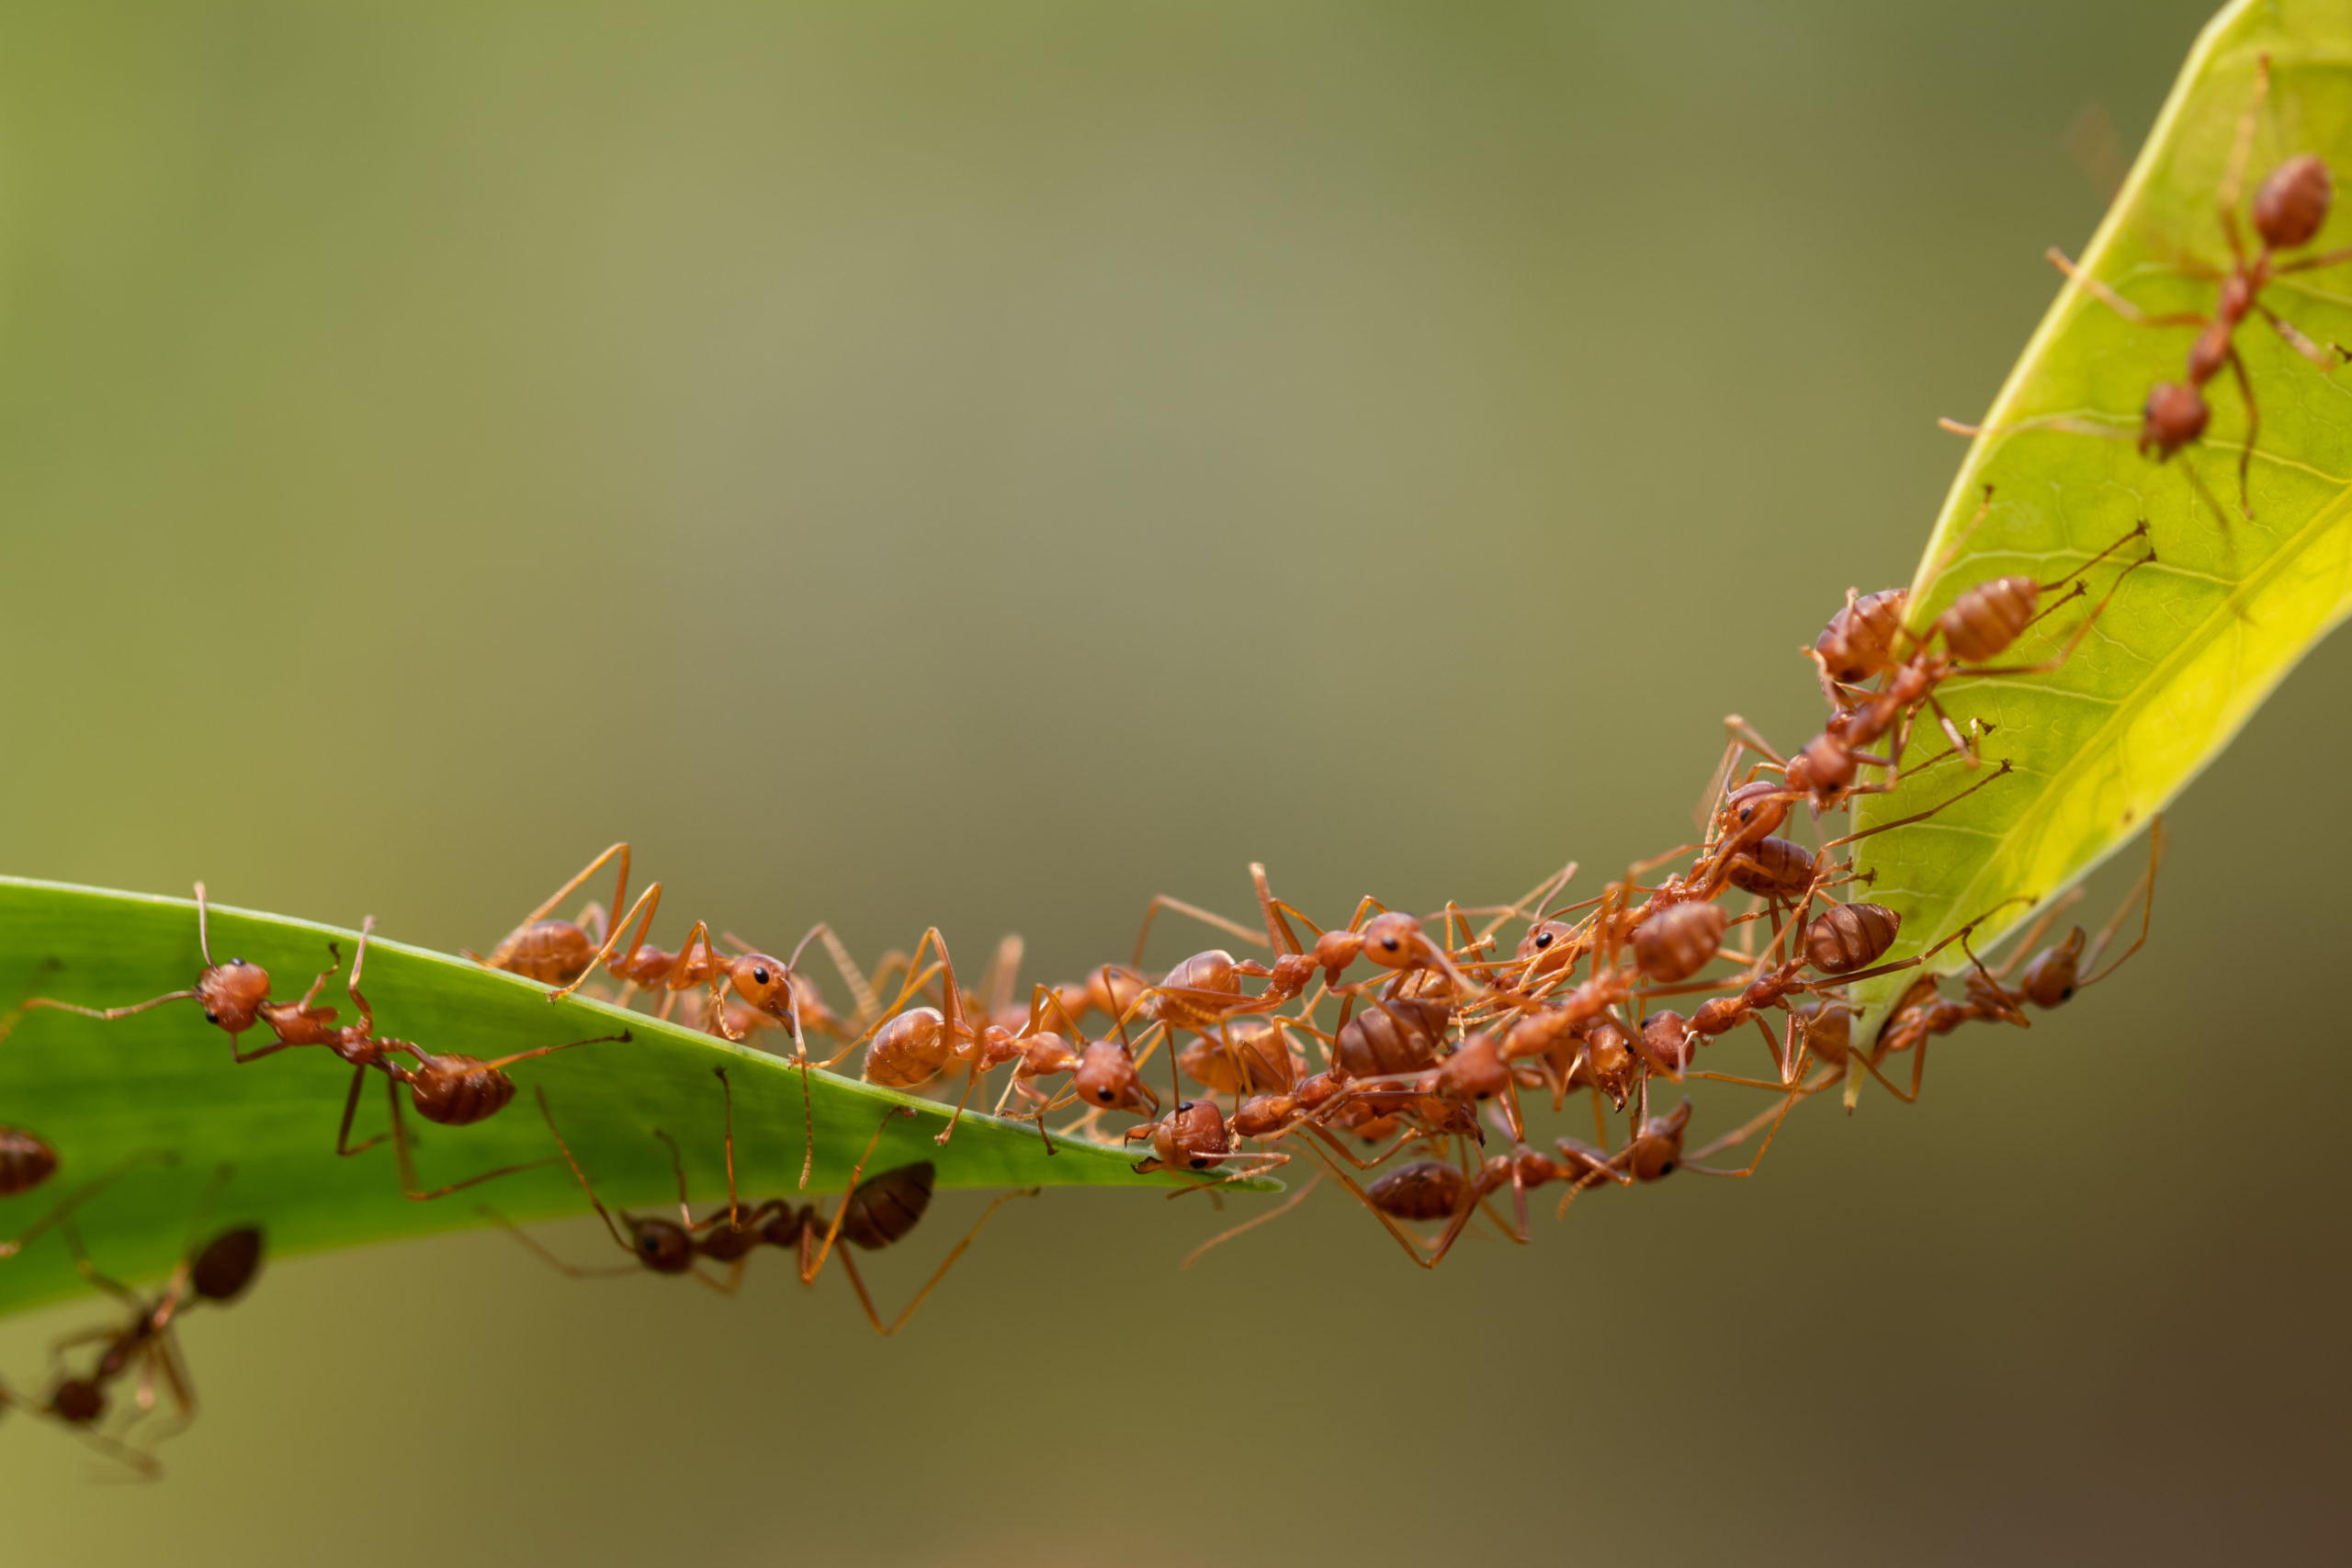
\includegraphics[trim={0 0cm 0 5cm}, clip, width=0.99\textwidth]{fig/0_ant-bridge.jpg}
    \caption{Esta fotografía ilustra cómo las hormigas son capaces de organizarse en una estructura entrelazada, utilizando sus cuerpos para formar un puente que les permite superar obstáculos y llegar a su destino de manera eficiente.}
    \label{fig:enjambre_naturaleza}
\end{figure}

De forma muy similar, en robótica nos referimos a un sistema descentralizado compuesto por múltiples robots poco sofisticados que, trabajando en equipo, logran generar una serie de \textbf{comportamientos colectivos} que permiten mejorar el rendimiento individual de cada agente. Este tipo de sistemas son muy interesantes y poderosos, no obstante, plantean una dificultad logística lo suficientemente significativa como para ser considerados actualmente como uno de los 10 grandes retos actuales en robótica según \textit{Science Robotics} \cite{10challenges}.

%(ver \autoref{fig:10challenges}).

En función de la finalidad para la que el sistema esté destinado, este gran reto se suele descomponer en numerosos problemas que también pueden llegar a ser bastante complejos. A nivel individual, podemos querer que cada individuo sea capaz percibir el medio, detectar la presencia de vecinos o seguir caminos. Mientras que a nivel de colectivo, se puede pensar en algoritmos distribuidos que permitan controlar movimientos en formación \cite{complex_laplacian}, realizar localización relativa \cite{relative_location}, evitar colisiones o buscar la fuente de un campo escalar. Al igual que en la naturaleza, todas estas tareas tan fundamentales pueden ser llevadas a cabo mediante una \emph{interacción local entre robots basada en las cuatro C's} \cite{resilient_swarm}: \textbf{coordinación}, \textbf{cooperación}, \textbf{colaboración} y \textbf{competición}.

\newpage
% \begin{figure}[h]
%     \centering
%     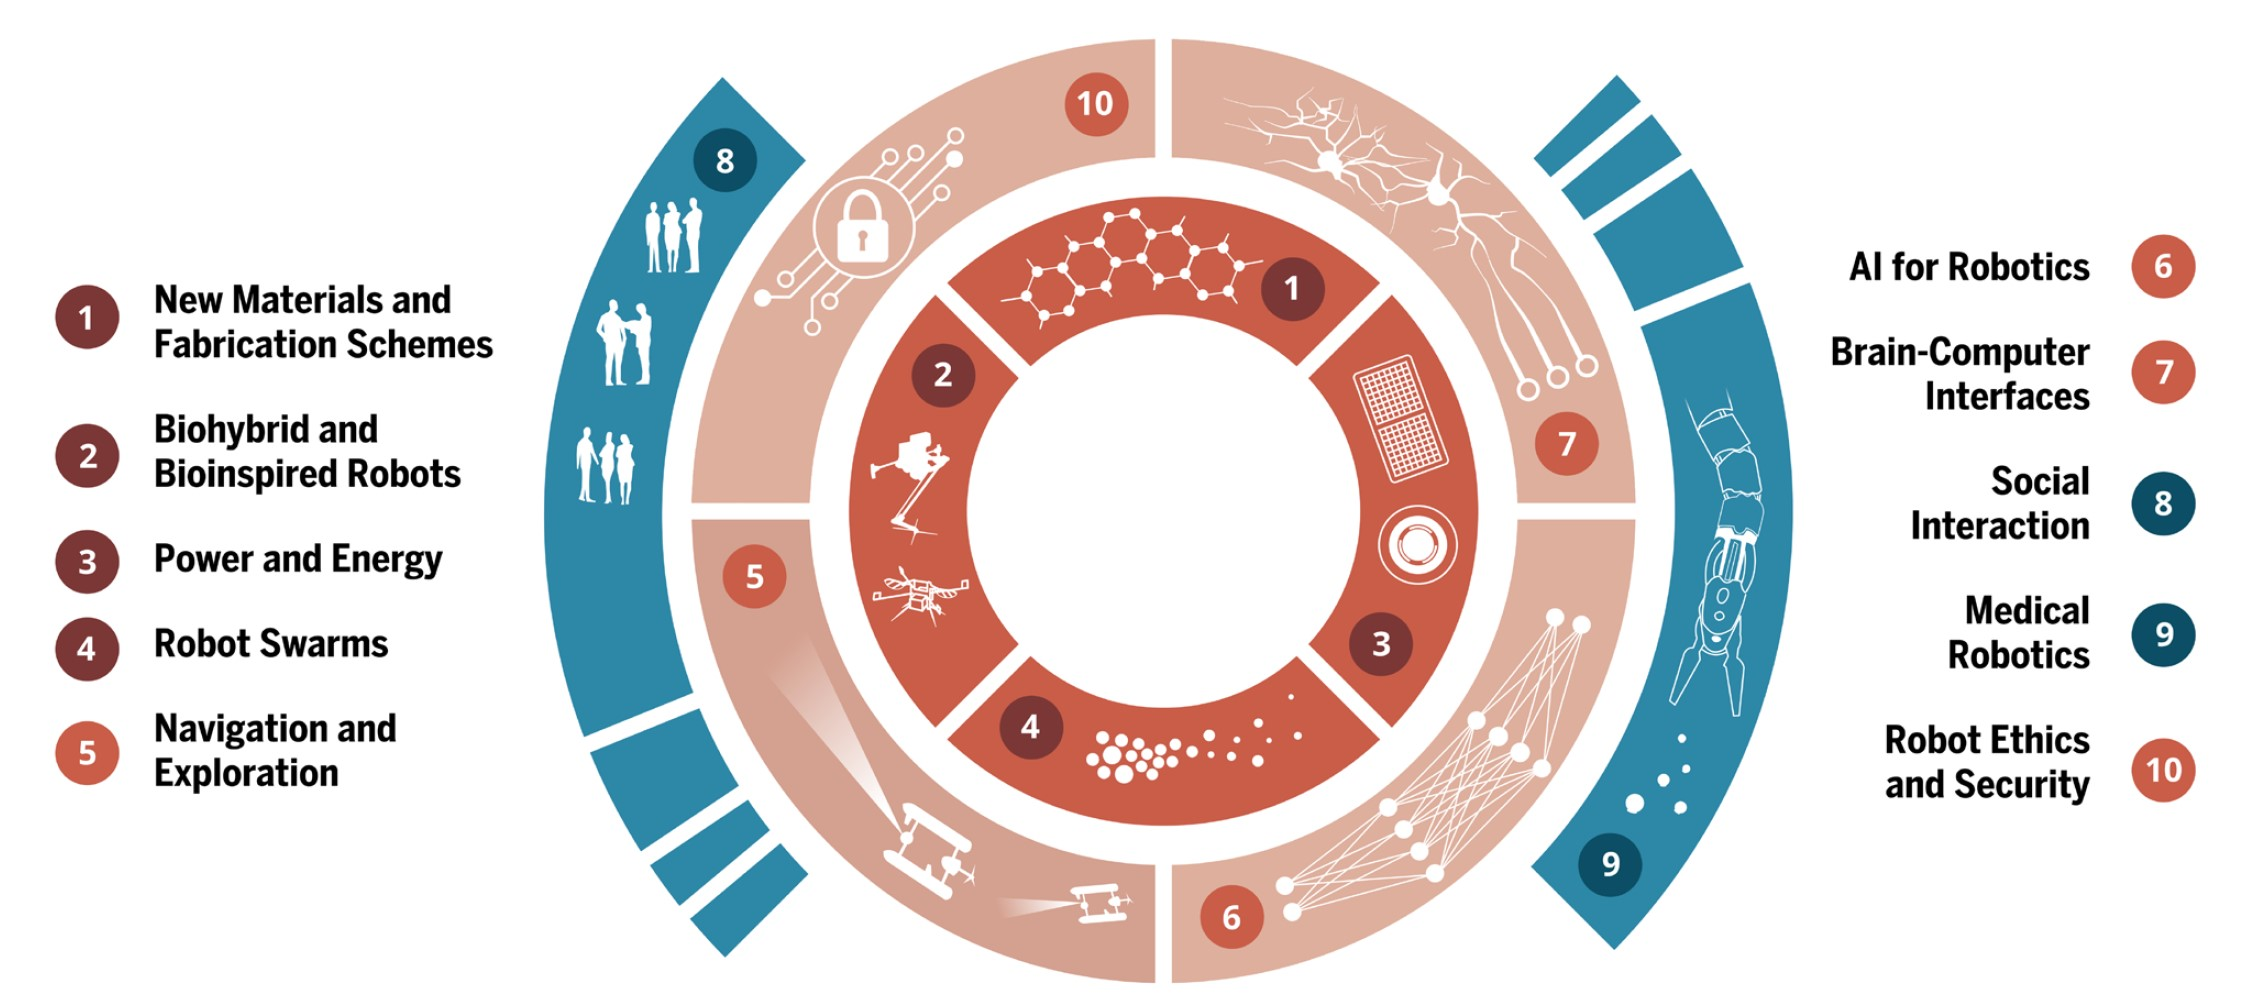
\includegraphics[trim={0 -1cm 0 -1cm}, clip, width=0.9\textwidth]{fig/1_10challenges.jpg}
%     \caption{Los 10 grandes retos actuales en robótica según \textit{Science Robotics} \cite{10challenges}.}
%     \label{fig:10challenges}
% \end{figure}

En este campo de la robótica siempre se habla sobre alcanzar la autonomía o \textbf{inteligencia de enjambre}, no obstante, no se suelen encontrar las técnicas más comunes de IA (Inteligencia Artificial), como lo son aquellas basadas en ML (\textit{Machine Learning}) o DP (\textit{Deep Learning}). Todas las metodologías que han demostrado rendir adecuadamente se basan reglas heurísticas, lógica difusa o teoría de control. Esto es algo que cobra bastante sentido cuando pensamos que en robótica, especialmente cuando hablamos de sistemas GNC (Guiado, Navegación y Control), lo que se suele buscar son algoritmos que aporten respuestas deterministas y altamente explicables. Este trabajo se centrará principalmente en técnicas de control basadas en análisis rigurosos y formales, pues por su naturaleza pueden llegar a ser más \textbf{robustas} y \textbf{resilientes} que otros métodos basados en reglas o comportamientos simples. Este tipo de garantías son necesarias en el caso de misiones consideradas ''criticas'' o que requieran de persistencia en el tiempo, conocidas como 24/7.

%%%%%%%%%%%%%%%%%%%%%%%%%%%%%%%%%%%%%
% Objetivos    %
%%%%%%%%%%%%%%%%

\subsection{Objetivos}

El fin principal de este trabajo es coordinar a un enjambre de robots mediante algoritmos GNC. Para lograrlo, se tendrán que alcanzar los siguientes objetivos específicos:

\begin{enumerate}
    \setlength\itemsep{1em}

    \item Desarrollar un algoritmo para la coordinación de vehículos terrestres garantizando la ausencia de colisiones.
    %Desarrollar un algoritmo un algoritmo basado en CBFs (\textit{Control Barrier Functions}) para garantizar la ausencia de colisiones entre vehículos en un sistema de seguimiento de caminos basado en GVFs (\textit{Guiding Vector Fields}).
    
    \item Implementar el algoritmo anterior en los sistemas empotrados de un enjambre robótico, de manera que todos los robots sean capaces de coordinarse de forma autónoma, sin la intervención de sistemas externos. %Para lograr este objetivo, se construirá una flota de \textit{rovers} de radio control equipados con la electrónica necesaria para alojar sistemas GNC.

    \item Desarrollar un algoritmo de búsqueda de fuentes en campos escalares para enjambres de robots que sea resiliente, distribuido y escalable.
\end{enumerate}

Dado que la presencia de garantías formales es uno de los puntos fuertes en teoría de control, todos los resultados matemáticos desarrollados en este trabajo serán demostrados y validados de forma numérica o experimental. 

%%%%%%%%%%%%%%%%%%%%%%%%%%%%%%%%%%%%%
% Organización    %
%%%%%%%%%%%%%%%%%%%

\subsection{Organización}

Una vez introducido el TFM y planteados sus objetivos, se presentarán dos metodologías distintas. Cada una de ellas, se focalizará en resolver un problema completamente distinto, por lo que ambas contarán con sus propias secciones de fundamentos teóricos, exposición de resultados, verificación numérica/experimental y conclusión. Una vez se haya terminado de hablar sobre ambas metodologías, en las últimas páginas de este trabajo se podrá encontrar la conclusión final y la sección de referencias.

%A lo largo de este trabajo se introducirán dos metodologías. En la primera (seccion x) se introducirá . Cada una de ellas presentará una sección de

%%%%%
%Este trabajo se centrará en desarrollar e integrar los algoritmos planteados anteriormente. En cada caso, se realizará una revisión  bibliográfica del estado del arte para, posteriormente, exponer, explicar y ampliar los resultados que mejor se adapten a la casuística y objetivos de este proyecto. Ha de tenerse en cuenta que todos los algoritmos desarrollados pretenden construir un sistema GNC, de modo que deberán de contar con ciertas garantías matemáticas. Por esta razón, en caso de que no existan, se realizarán análisis formales sobre cada uno de ellos.

%En relación a la parte de integración, se describirá con detalle toda la plataforma hardware de los robots, y se propondrán distintas estrategias para implementar y coordinar cada uno de los sistemas GNC. Todo este trabajo se ha desarrollado bajo el marco del proyecto de software y hardware libre Paparazzi UAS \cite{github_pprz}, de modo que cualquier aportación a nivel de código se encontrará publicada en una rama de dicho proyecto gestionada por el autor de este trabajo \cite{github}.


%%%%%%%%%%%%%%%%%%%%%%%%%%%%%%%%%%%%%